% !TEX root = main.tex
\section{Experiments}
\subsection{Data and human panel}\label{sec:data-human-protocol}\label{sec:veribench-overview}
We evaluate candidate--gold pairs from \textsc{VeriBench}~\citep{miranda2026veribench}.
One annotator supplied holistic ratings on a $0$--$5$ scale in two passes, pass1 with a stricter rubric and pass2 with a more lenient rubric.
The collection covered 75 pairs from 25 problems with three agent generations per problem.
One gold filename could not be resolved, leaving 72 analyzed pairs from 24 problems.
We report each pass and the archived averaged-label view; they are two judgments by one person, not independent annotators.
Inter-pass agreement is Spearman $0.249$, quadratic-weighted $\kappa=0.372$, and mean absolute error $0.771$ on the shared pairs (Appendix~\ref{app:exp16-exp17}).
These statistics describe label disagreement; they do not establish an upper bound on judge agreement.
The original written rubric was not recovered, so we cannot reconstruct every annotation instruction.

This panel is the \emph{validation set}: it informed index-form selection, repeat aggregation, the threshold, and the prompt panel, so correlations on it are optimistic.
The fixed equal-weight $\mathrm{TI}_{\mathrm{var}}$ has no training set.
A separate weight-tuned comparison uses these same pairs, and no analysis constitutes a test-set result.
For each judge, artifact-level agreement is the Spearman correlation between its scores and the human ratings on the same analyzed pairs.
We then ask whether the index orders configurations by that agreement.

\subsection{Property checks on GPT-5.3-Codex}\label{sec:property-results}
Figure~\ref{fig:judge_sanity_checks} summarizes the 24-problem panel for three Codex prompts.
Their mean scores decrease as bug-ladder edits accumulate, but averages conceal local reversals.
The strict prompt reverses on four of 24 ladders, whereas the baseline and checklist prompts have no reversals (Table~\ref{tab:codex_configs}).
The archived alpha probes produce the largest score changes among the four rewrite types, but their generator can produce malformed Lean text.
The baseline and checklist prompts assign them zero mean score, despite near-maximum scores for the other rewrites.
The strict prompt gives alpha-renamed artifacts a mean score of $0.179$.
Appendix~\ref{app:failure-diagnostics} retains the per-configuration diagnostics and the corresponding Claude Opus summary.

\begin{figure}[t]
\centering
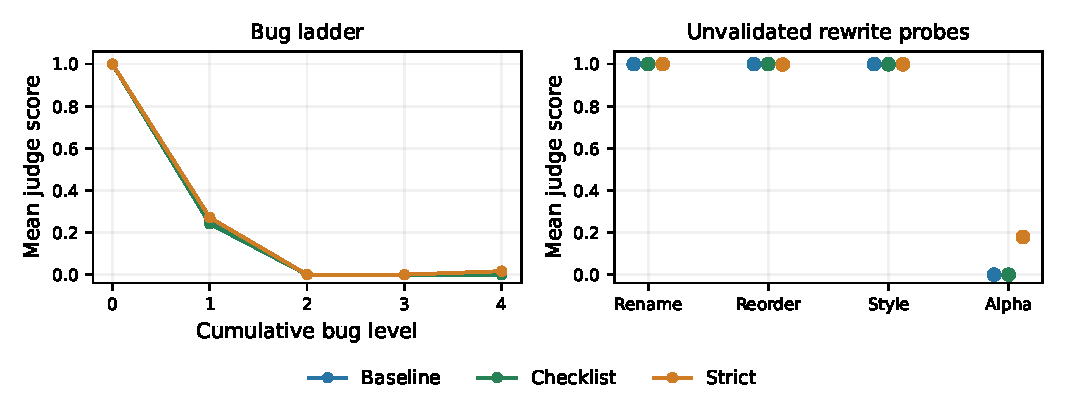
\includegraphics[width=\linewidth]{figures/codex_property_checks.pdf}
\caption{Mean scores fall with cumulative bug edits, but malformed alpha probes sharply change the Codex judges' scores.
Each point averages median scores over 24 problems, with three calls per problem and prompt; these are descriptive means, not uncertainty intervals.
Local reversals remain visible in Table~\ref{tab:codex_configs}.}
\label{fig:judge_sanity_checks}
\end{figure}

\paragraph{Alpha-renaming and a canonicalization proxy.}
The historical alpha routine can duplicate the assignment marker and rename signature variables without updating the proof body.
Its score drops therefore cannot establish a failure of invariance under valid alpha-renaming.
A post-hoc proxy replaces each judge's alpha scores with its median score under style edits.
Across the eight Codex-panel configurations, this lowers the mean per-judge standard deviation across identity-probe scores from $0.250$ to $0.070$.
This manipulation changes recorded scores rather than the judge's inputs.
A real fix must rescore canonicalized text and verify that the transformation preserves meaning.

\paragraph{Coverage of P3.}
The eight-configuration panel contains identity rewrites and bug ladders but no missing-specification ladders.
Consequently, it cannot establish which association P3 has with human agreement.
We retain P3 as a proposed part of the protocol, without attributing the bug-ladder statistics below to it.

\subsection{The index tracks judge-level human agreement on the validation set}\label{sec:tivar_cross_model_results}\label{sec:validation-human-alignment}
The three primary families are GPT-5.3-Codex, Claude Opus 4.7, and Qwen3-Coder.
Each eight-configuration panel contains three semantic prompts, a deliberately lexical prompt on the same model, two GPT-4o-mini prompts, edit distance, and a random control.
These are family panels with shared controls, not eight independent models per family.
The frozen model identifiers and complete main-panel prompts appear in Appendix~\ref{app:judge-prompts}.
Scores are medians over three repeated calls for language-model judges; Codex-panel controls use nine repeats, and the other panels use three.

Figure~\ref{fig:tivar_cross_model_avg} uses the fixed equal-weight index in Equation~\ref{eq:tivar}.
Its judge-level Spearman association is positive for each primary family and label view (Table~\ref{tab:tivar_cross_model_results}).
For Codex, averaged-label Pearson and Kendall associations are $0.868$ and $0.643$, respectively.
The Codex bootstrap intervals are wide, and the resampling does not correct for the earlier protocol selection.
Pass-to-pass differences also matter: Qwen's Spearman association changes from $0.476$ on pass1 to $0.857$ on pass2.
With eight configurations and disagreeing label passes, these estimates support a descriptive association rather than a precise or portable effect size.

\begin{figure}[t]
\centering
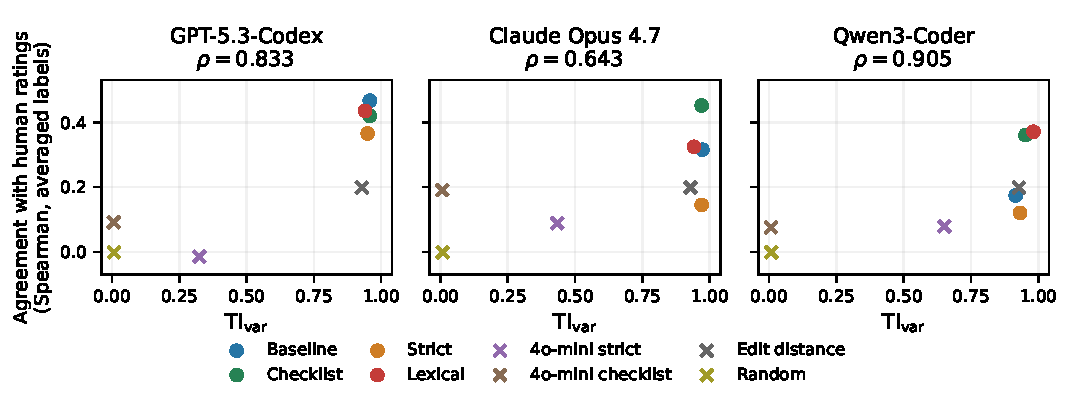
\includegraphics[width=\linewidth]{figures/judge_agreement_fixed_index.pdf}
\caption{The fixed equal-weight index has a positive association with human agreement in each primary family, but high index values do not rule out lexical judges.
Each point is one configuration; the vertical axis is its Spearman agreement with averaged human labels on 72 pairs.
Panel titles report the correlation across eight configurations; Table~\ref{tab:tivar_cross_model_results} gives Codex uncertainty.}
\label{fig:tivar_cross_model_avg}
\end{figure}

\begin{table}[t]
\centering\small
\begin{tabular}{@{}lrrrrrr@{}}
\toprule
& \multicolumn{4}{c}{Averaged labels} & \multicolumn{2}{c}{$\mathrm{TI}_{\mathrm{var}}$ by pass} \\
\cmidrule(lr){2-5}\cmidrule(lr){6-7}
Family & $v1$ & $v2$ & $\mathrm{GM}_{.4,.6}$ & $\mathrm{TI}_{\mathrm{var}}$ & pass1 & pass2 \\
\midrule
Codex & 0.762 & 0.476 & 0.857 & 0.833 & 0.905 & 0.738 \\
Claude Opus & 0.429 & 0.143 & 0.714 & 0.643 & 0.810 & 0.595 \\
Qwen3-Coder & 0.524 & 0.500 & 0.786 & 0.905 & 0.476 & 0.857 \\
\midrule
\multicolumn{4}{l}{Codex $\mathrm{TI}_{\mathrm{var}}$: 95\% interval} & $[0.24,1.00]$ & $[0.41,1.00]$ & $[0.11,1.00]$ \\
\multicolumn{4}{l}{Codex $\mathrm{TI}_{\mathrm{var}}$: permutation $p$} & 0.017 & 0.005 & 0.045 \\
\bottomrule
\end{tabular}
\caption{The fixed index is competitive with a two-component geometric comparison whose weights were selected on pass1.
Entries are Spearman correlations between each index and judge-level human agreement on the validation set, with eight configurations per family.
Codex intervals and permutation probabilities use 10{,}000 resamples and permutations, seed 42; corresponding intervals for the other families are not reported.
Appendix~\ref{app:index-definitions} defines all indices.}
\label{tab:tivar_cross_model_results}\label{tab:cross_model_index_compare_avg}
\end{table}

\paragraph{Human agreement alone can miss a bad judge.}
The lexical prompt, \texttt{BAD\_STRINGY}, explicitly instructs the model to ignore theorem meaning and grade textual overlap.
On the Codex panel, its human agreement of $0.435$ lies among the semantic prompts' values, $0.365$--$0.466$.
Yet it reverses on 20 of 24 bug ladders (Table~\ref{tab:codex_configs}).
The index ranks it below the three semantic prompts, but its value remains $0.940$; edit distance also scores highly at $0.928$.
In the Qwen panel, the lexical configuration has the highest index value, $0.982$.
The failure report therefore carries information that both human agreement and the scalar can miss.
No validated cutoff on $\mathrm{TI}_{\mathrm{var}}$ establishes that a judge is acceptable.

\begin{table}[t]
\centering\small
\begin{tabular}{@{}lrrr@{}}
\toprule
Codex-panel configuration & Human $\rho$ (avg) & $\mathrm{TI}_{\mathrm{var}}$ & Ladders with reversals \\
\midrule
Baseline prompt & 0.466 & 0.958 & 0/24 \\
Checklist prompt & 0.419 & 0.958 & 0/24 \\
Strict prompt & 0.365 & 0.950 & 4/24 \\
Lexical prompt & 0.435 & 0.940 & 20/24 \\
GPT-4o-mini, strict & $-0.014$ & 0.324 & 18/24 \\
GPT-4o-mini, checklist & 0.092 & 0.007 & 16/24 \\
Edit distance & 0.199 & 0.928 & 24/24 \\
Random & $-0.001$ & 0.008 & 24/24 \\
\bottomrule
\end{tabular}
\caption{The lexical judge agrees with humans despite frequent bug-ladder reversals, and the scalar index penalizes it only slightly.
A reversal is any local score increase as cumulative edits are added; the diagnostic uses the recorded repeat-aggregated scores.}
\label{tab:codex_configs}
\end{table}

\paragraph{Choice of index.}
The two-component geometric comparison is numerically higher than $\mathrm{TI}_{\mathrm{var}}$ for Codex and Opus on averaged labels (Table~\ref{tab:tivar_cross_model_results}).
It uses bug monotonicity and decision stability with weights $0.4$ and $0.6$, selected on pass1, rather than fixed equal weights.
We retain $\mathrm{TI}_{\mathrm{var}}$ for its explicit variance penalties and positive associations across the primary families and passes, not because these data establish its superiority.
A separate search over six component weights gives cross-pass associations of $0.810$ and $0.786$ on the same pairs (Appendix~\ref{app:moved-results}).
The pass1-selected geometric form reaches $0.769$ on an expanded 13-configuration panel, with a 95\% interval of $[0.34,0.95]$ (Appendix~\ref{app:expanded-panel}).
Neither comparison provides a held-out estimate.
A separate Leanstral panel has averaged-label association $-0.095$ for the fixed index (Appendix~\ref{app:negative-results}), so the positive result does not hold for every recorded family.

\paragraph{Weight and normalization sensitivity.}
Recomputing the fixed index on a local grid of weight triples gives averaged-label Spearman ranges of $0.738$--$0.857$ for Codex, $0.643$--$0.714$ for Opus, and $0.881$--$0.976$ for Qwen.
This analysis uses only committed component vectors and keeps their normalization fixed (Appendix~\ref{app:weight-sensitivity}).
It does not assess sensitivity to changing the normalization panel.
We do not report leave-one-family-out transfer: the panels share controls and normalize separately, so pooling their scores would not constitute an independent family test.

\paragraph{Which measured statistics matter.}
Among the recorded diagnostics, weak monotonicity on bug ladders has the largest association with human agreement on each label view (Table~\ref{tab:property_assoc}).
It measures the absence of local increases; bug-rank correlation measures the overall direction.
The archived field name \texttt{P3\_weak\_mono} refers to this bug statistic, not to the P3 missing-specification property.
Identity-rewrite scores and repeat decision stability have weaker or inconsistent associations.
Only the weak-monotonicity statistic on pass2 and averaged labels has an unadjusted permutation $p<0.05$; these component comparisons are exploratory.

\begin{table}[t]
\centering\small
\begin{tabular}{@{}lrrr@{}}
\toprule
Measured diagnostic & pass1 & pass2 & avg \\
\midrule
Mean identity-rewrite score & $-0.21$ (0.62) & 0.02 (0.98) & $-0.02$ (0.98) \\
Bug-rank monotonicity & 0.60 (0.13) & 0.67 (0.08) & 0.71 (0.06) \\
Bug weak monotonicity & 0.63 (0.11) & 0.78 (0.03) & 0.75 (0.04) \\
Repeat decision stability & 0.47 (0.24) & $-0.23$ (0.57) & 0.14 (0.76) \\
\bottomrule
\end{tabular}
\caption{Bug weak monotonicity has the largest observed association among the measured diagnostics; this table contains no P3 missing-specification result.
Entries are Spearman correlations with human agreement across eight Codex-panel configurations; unadjusted permutation probabilities appear in parentheses.}
\label{tab:property_assoc}
\end{table}

\paragraph{Artifact-score threshold.}
A historical sweep of the artifact-score threshold from $0.60$ to $0.85$ lowers the observed decision-flip rate from $0.058$ to $0.046$ and pass rate from $0.583$ to $0.536$ (Appendix Table~\ref{tab:exp13_threshold_sweep}).
The selected threshold is $0.85$, which has the lowest observed flip rate in that sweep.
This thresholds $J_\theta(x,g)$, not the judge-level index, and measures repeatability rather than correctness of the accepted artifacts.
